\documentclass[11pt,a4paper]{article}
\usepackage[margin=0.8in]{geometry}
\usepackage{tikz}
\usepackage{pgf-umlcd}
\usepackage{fontspec}
\usepackage{xcolor}
\usepackage{amsfonts}
\usepackage{amsmath}
\usepackage{listings}
\usepackage{array}

% Configure emoji font for XeLaTeX (vector-based for better compatibility)
\newfontfamily\emojifont{Segoe UI Emoji}[
    Scale=1.0
]

% Create convenient emoji command
\newcommand{\emoji}[1]{{\emojifont #1}}

\usetikzlibrary{shapes,arrows,positioning,fit,backgrounds,decorations.pathmorphing,calc,shadows,matrix}

\title{PeiDocker Terminal GUI - Component Specifications}
\author{Claude Code}
\date{\today}

\definecolor{primaryblue}{RGB}{51,122,183}
\definecolor{successgreen}{RGB}{92,184,92}
\definecolor{warningorange}{RGB}{240,173,78}
\definecolor{dangered}{RGB}{217,83,79}
\definecolor{lightgray}{RGB}{248,248,248}
\definecolor{darkgray}{RGB}{85,85,85}
\definecolor{infoblue}{RGB}{91,192,222}
\definecolor{purpleaccent}{RGB}{149,117,205}

\tikzset{
    % Component frame styles
    component/.style={
        rectangle, draw=primaryblue, thick, fill=lightgray!20,
        minimum width=6cm, minimum height=3cm,
        rounded corners=3pt
    },
    widget/.style={
        rectangle, draw=successgreen, fill=successgreen!10,
        minimum width=4cm, minimum height=1.5cm,
        rounded corners=2pt
    },
    interface/.style={
        rectangle, draw=purpleaccent, fill=purpleaccent!10,
        text width=8cm, minimum height=2cm,
        rounded corners=3pt
    },
    codeblock/.style={
        rectangle, draw=darkgray, fill=darkgray!10,
        text width=7cm, font=\ttfamily\footnotesize,
        rounded corners=2pt
    }
}

\lstset{
    basicstyle=\ttfamily\footnotesize,
    backgroundcolor=\color{lightgray!30},
    frame=single,
    breaklines=true,
    showstringspaces=false,
    language=Python
}

\begin{document}

\maketitle

\section{Component Architecture Overview}

This document specifies the individual UI components and widgets that comprise the PeiDocker Terminal GUI. Each component is designed for reusability across both Simple and Advanced modes, following the Textual framework patterns.

\subsection{Component Hierarchy}

\begin{figure}[htbp]
\centering
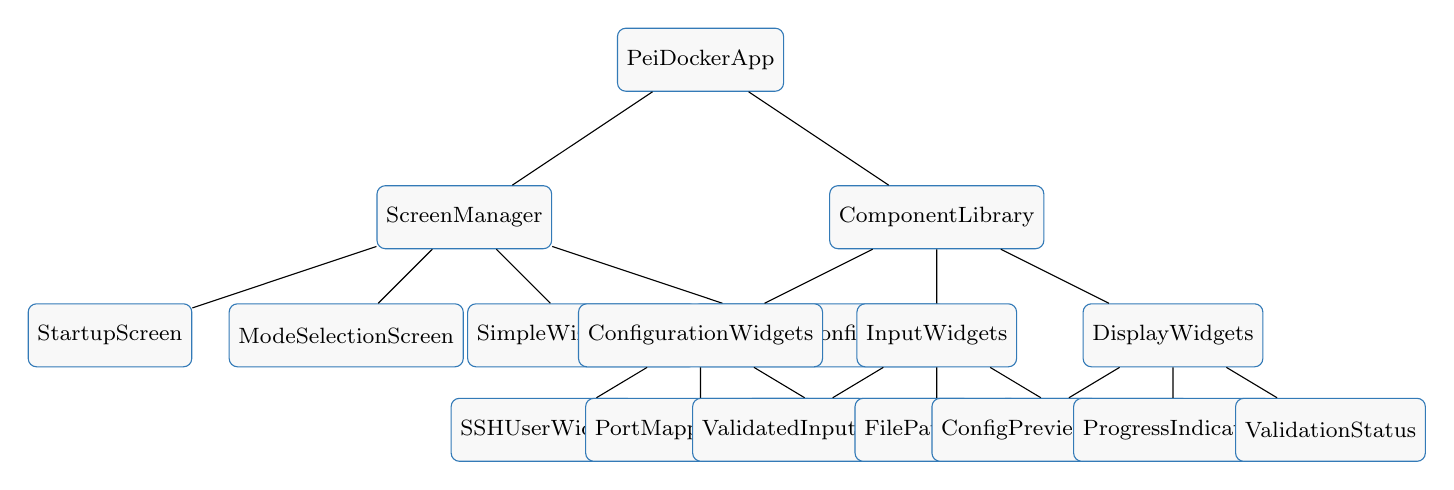
\begin{tikzpicture}[
    level 1/.style={sibling distance=6cm, level distance=2cm},
    level 2/.style={sibling distance=3cm, level distance=1.5cm},
    level 3/.style={sibling distance=2cm, level distance=1.2cm},
    every node/.style={
        rectangle, draw=primaryblue, fill=lightgray, 
        text centered, rounded corners=3pt,
        font=\footnotesize, minimum height=0.8cm
    }
]

\node {PeiDockerApp}
    child { node {ScreenManager}
        child { node {StartupScreen} }
        child { node {ModeSelectionScreen} }
        child { node {SimpleWizardScreen} }
        child { node {AdvancedConfigScreen} }
    }
    child { node {ComponentLibrary}
        child { node {ConfigurationWidgets}
            child { node {SSHUserWidget} }
            child { node {PortMappingWidget} }
            child { node {EnvironmentWidget} }
        }
        child { node {InputWidgets}
            child { node {ValidatedInput} }
            child { node {FilePathInput} }
            child { node {MultiSelectInput} }
        }
        child { node {DisplayWidgets}
            child { node {ConfigPreview} }
            child { node {ProgressIndicator} }
            child { node {ValidationStatus} }
        }
    };

\end{tikzpicture}
\caption{Component Architecture Hierarchy}
\end{figure}

\section{Base Component Classes}

\subsection{BaseConfigWidget}

\begin{figure}[htbp]
\centering
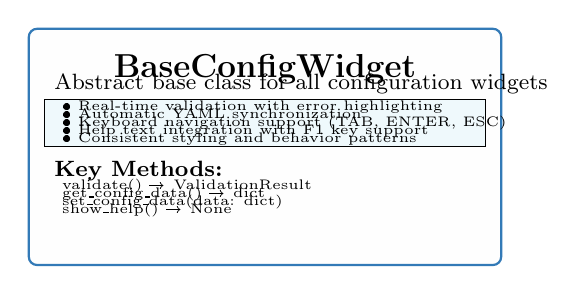
\begin{tikzpicture}

% Component frame
\node[component] (frame) at (0,0) {};
\node[anchor=north, font=\large\bfseries] at (0,1.3) {BaseConfigWidget};

% Widget structure
\node[anchor=west, font=\footnotesize] at (-2.8,0.8) {Abstract base class for all configuration widgets};

% Key features box
\draw[fill=infoblue!10] (-2.8,0) rectangle (2.8,0.6);
\node[anchor=west, font=\tiny] at (-2.7,0.5) {• Real-time validation with error highlighting};
\node[anchor=west, font=\tiny] at (-2.7,0.4) {• Automatic YAML synchronization};
\node[anchor=west, font=\tiny] at (-2.7,0.3) {• Keyboard navigation support (TAB, ENTER, ESC)};
\node[anchor=west, font=\tiny] at (-2.7,0.2) {• Help text integration with F1 key support};
\node[anchor=west, font=\tiny] at (-2.7,0.1) {• Consistent styling and behavior patterns};

% Methods section
\node[anchor=west, font=\footnotesize\bfseries] at (-2.8,-0.3) {Key Methods:};
\node[anchor=west, font=\tiny] at (-2.7,-0.5) {validate() → ValidationResult};
\node[anchor=west, font=\tiny] at (-2.7,-0.6) {get\_config\_data() → dict};
\node[anchor=west, font=\tiny] at (-2.7,-0.7) {set\_config\_data(data: dict)};
\node[anchor=west, font=\tiny] at (-2.7,-0.8) {show\_help() → None};

\end{tikzpicture}
\caption{BaseConfigWidget Specification}
\end{figure}

\begin{lstlisting}[caption={BaseConfigWidget Implementation}, label={lst:base_widget}]
from textual.widget import Widget
from textual.reactive import reactive
from abc import ABC, abstractmethod
from typing import Dict, Any, Optional

class BaseConfigWidget(Widget, ABC):
    """Abstract base class for all configuration widgets."""
    
    # Reactive properties for real-time updates
    config_data: reactive[Dict[str, Any]] = reactive({})
    validation_errors: reactive[list] = reactive([])
    is_modified: reactive[bool] = reactive(False)
    
    def __init__(self, config_key: str, **kwargs):
        super().__init__(**kwargs)
        self.config_key = config_key
        self.help_text = ""
        
    @abstractmethod
    def validate(self) -> Dict[str, Any]:
        """Validate current widget data and return validation result."""
        pass
        
    @abstractmethod
    def get_config_data(self) -> Dict[str, Any]:
        """Get current configuration data for YAML generation."""
        pass
        
    @abstractmethod
    def set_config_data(self, data: Dict[str, Any]) -> None:
        """Set configuration data from loaded YAML."""
        pass
        
    def on_mount(self) -> None:
        """Called when widget is mounted to the screen."""
        self.set_focus()
        
    def action_show_help(self) -> None:
        """Show help dialog for this widget (F1 key)."""
        self.app.show_help_dialog(self.help_text)
        
    def watch_config_data(self, new_data: Dict[str, Any]) -> None:
        """Called when config_data changes - trigger validation."""
        self.validation_errors = self.validate()
        self.is_modified = True
        self.app.update_yaml_preview()
\end{lstlisting}

\section{Input Widget Components}

\subsection{ValidatedInput Widget}

\begin{figure}[htbp]
\centering
\begin{tikzpicture}

\node[widget] at (0,0) {};
\node[anchor=north, font=\bfseries] at (0,0.6) {ValidatedInput};

% Visual representation
\draw[fill=white] (-1.8,-0.3) rectangle (1.8,0);
\node[anchor=west, font=\ttfamily\tiny] at (-1.7,-0.15) {ubuntu:24.04};

% Validation indicator
\draw[fill=successgreen] (1.6,-0.25) rectangle (1.75,-0.05);
\node[font=\tiny] at (1.9,-0.15) {\emoji{✓}};

% Error state example
\draw[fill=white] (-1.8,-0.8) rectangle (1.8,-0.5);
\node[anchor=west, font=\ttfamily\tiny, color=dangered] at (-1.7,-0.65) {invalid-image-name!@\#};
\draw[fill=dangered] (1.6,-0.75) rectangle (1.75,-0.55);
\node[font=\tiny, color=white] at (1.9,-0.65) {\emoji{✗}};

\end{tikzpicture}
\caption{ValidatedInput Widget States}
\end{figure}

\begin{lstlisting}[caption={ValidatedInput Implementation}]
from textual.widgets import Input
from textual.validation import ValidationResult, Validator
import re

class ValidatedInput(Input):
    """Input widget with real-time validation and visual feedback."""
    
    def __init__(self, 
                 placeholder: str = "",
                 validators: list[Validator] = None,
                 **kwargs):
        super().__init__(placeholder=placeholder, **kwargs)
        self.validators = validators or []
        
    def validate_value(self, value: str) -> ValidationResult:
        """Run all validators on the current value."""
        for validator in self.validators:
            result = validator.validate(value)
            if not result.is_valid:
                return result
        return ValidationResult.success()
        
    def on_input_changed(self, event) -> None:
        """Called when input value changes."""
        validation = self.validate_value(self.value)
        
        # Update visual state based on validation
        if validation.is_valid:
            self.add_class("valid")
            self.remove_class("invalid")
        else:
            self.add_class("invalid")
            self.remove_class("valid")
            
        # Emit validation event for parent widgets
        self.post_message(
            ValidationEvent(self, validation)
        )

# Common validators
class DockerImageValidator(Validator):
    """Validates Docker image name format."""
    
    def validate(self, value: str) -> ValidationResult:
        pattern = r'^[a-z0-9]+([-._][a-z0-9]+)*(/[a-z0-9]+([-._][a-z0-9]+)*)*(:[\w][\w.-]*)?$'
        if re.match(pattern, value.lower()):
            return ValidationResult.success()
        return ValidationResult.failure("Invalid Docker image name format")

class PortValidator(Validator):
    """Validates port numbers (1-65535)."""
    
    def validate(self, value: str) -> ValidationResult:
        try:
            port = int(value)
            if 1 <= port <= 65535:
                return ValidationResult.success()
            return ValidationResult.failure("Port must be between 1 and 65535")
        except ValueError:
            return ValidationResult.failure("Port must be a valid number")
\end{lstlisting>

\subsection{FilePathInput Widget}

\begin{figure}[htbp]
\centering
\begin{tikzpicture}

\node[widget] at (0,0) {};
\node[anchor=north, font=\bfseries] at (0,0.6) {FilePathInput};

% File path input with browse button
\draw[fill=white] (-1.8,-0.2) rectangle (1.2,0.1);
\node[anchor=west, font=\ttfamily\tiny] at (-1.7,-0.05) {/home/user/.ssh/id_rsa};

% Browse button
\draw[fill=primaryblue!30] (1.3,-0.2) rectangle (1.8,0.1);
\node[font=\tiny] at (1.55,-0.05) {\emoji{📁}};

% Special syntax support
\node[anchor=west, font=\tiny] at (-1.8,-0.4) {Supports: ~ (auto-discovery), absolute paths, relative paths};

% File existence indicator
\draw[fill=successgreen] (-1.9,-0.15) rectangle (-1.85,0.05);
\draw[fill=warningorange] (-1.9,-0.6) rectangle (-1.85,-0.4);

\end{tikzpicture}
\caption{FilePathInput Widget with Browse Support}
\end{figure}

\begin{lstlisting}[caption={FilePathInput Implementation}]
from textual.widgets import Input, Button
from textual.containers import Horizontal
from pathlib import Path
import os

class FilePathInput(Horizontal):
    """File path input with browse button and special syntax support."""
    
    def __init__(self, 
                 placeholder: str = "Enter file path or '~' for auto-discovery",
                 file_type: str = "file",  # "file" or "directory"
                 **kwargs):
        super().__init__(**kwargs)
        self.file_type = file_type
        
    def compose(self):
        yield Input(
            placeholder=self.placeholder,
            id="path_input"
        )
        yield Button("\emoji{📁}", id="browse_button", variant="primary")
        
    def on_mount(self):
        self.path_input = self.query_one("#path_input", Input)
        self.browse_button = self.query_one("#browse_button", Button)
        
    def on_input_changed(self, event) -> None:
        """Validate path and show existence status."""
        path_str = self.path_input.value
        
        if path_str == "~":
            # Special auto-discovery syntax
            self.add_class("auto-discovery")
        else:
            self.remove_class("auto-discovery")
            
            # Check if path exists
            try:
                path = Path(path_str).expanduser()
                if path.exists():
                    self.add_class("path-exists")
                    self.remove_class("path-missing")
                else:
                    self.add_class("path-missing")
                    self.remove_class("path-exists")
            except (OSError, ValueError):
                self.add_class("path-invalid")
                
    def on_button_pressed(self, event) -> None:
        """Open file browser dialog."""
        if event.button.id == "browse_button":
            self.app.open_file_dialog(
                file_type=self.file_type,
                callback=self.set_path
            )
            
    def set_path(self, path: str) -> None:
        """Set the selected path."""
        self.path_input.value = path
        
    @property
    def value(self) -> str:
        """Get the current path value."""
        return self.path_input.value
        
    @value.setter
    def value(self, path: str) -> None:
        """Set the path value."""
        self.path_input.value = path
\end{lstlisting>

\section{Configuration Widget Components}

\subsection{SSHUserWidget}

\begin{figure}[htbp]
\centering
\begin{tikzpicture}

\node[component] at (0,0) {};
\node[anchor=north, font=\large\bfseries] at (0,1.3) {SSHUserWidget};

% User configuration form
\node[anchor=west, font=\footnotesize] at (-2.8,0.8) {Username:};
\draw[fill=white] (-1.5,0.7) rectangle (0.5,0.9);
\node[anchor=west, font=\ttfamily\tiny] at (-1.4,0.8) {me};

\node[anchor=west, font=\footnotesize] at (-2.8,0.5) {Password:};
\draw[fill=white] (-1.5,0.4) rectangle (0.5,0.6);
\node[anchor=west, font=\ttfamily\tiny] at (-1.4,0.5) {••••••};

\node[anchor=west, font=\footnotesize] at (-2.8,0.2) {UID:};
\draw[fill=white] (-1.5,0.1) rectangle (-0.5,0.3);
\node[anchor=west, font=\ttfamily\tiny] at (-1.4,0.2) {1000};

% SSH Key section
\node[anchor=west, font=\footnotesize] at (-2.8,-0.1) {Public Key:};
\draw[fill=lightgray!50] (-1.5,-0.2) rectangle (0.5,0);
\node[anchor=west, font=\ttfamily\tiny] at (-1.4,-0.1) {~/.ssh/id_rsa.pub};

\node[anchor=west, font=\footnotesize] at (-2.8,-0.4) {Private Key:};
\draw[fill=lightgray!50] (-1.5,-0.5) rectangle (0.5,-0.3);
\node[anchor=west, font=\ttfamily\tiny] at (-1.4,-0.4) {~};

% Action buttons
\draw[fill=successgreen!30] (1,-0.1) rectangle (2.8,0.1);
\node[font=\tiny] at (1.9,0) {Generate Keys};

\draw[fill=primaryblue!30] (1,-0.4) rectangle (2.8,-0.2);
\node[font=\tiny] at (1.9,-0.3) {Validate Config};

\end{tikzpicture}
\caption{SSHUserWidget Configuration Interface}
\end{figure}

\begin{lstlisting}[caption={SSHUserWidget Implementation}]
from textual.containers import Vertical, Horizontal
from textual.widgets import Input, Button, Checkbox
from .base import BaseConfigWidget
from .file_path_input import FilePathInput

class SSHUserWidget(BaseConfigWidget):
    """Widget for configuring SSH user accounts."""
    
    def __init__(self, username: str = "", **kwargs):
        super().__init__(config_key="ssh_user", **kwargs)
        self.username = username
        self.help_text = """
SSH User Configuration:
- Username: System username for SSH access
- Password: Authentication password (avoid commas/spaces)
- UID: User ID (>= 1100 recommended to avoid conflicts)
- Public Key: SSH public key for key-based auth
- Private Key: SSH private key file
- Use '~' for automatic system key discovery
        """
        
    def compose(self):
        with Vertical():
            with Horizontal():
                yield Input(
                    placeholder="Username", 
                    value=self.username,
                    id="username"
                )
                yield Input(
                    placeholder="UID", 
                    value="1000",
                    id="uid"
                )
            
            yield Input(
                placeholder="Password",
                password=True,
                id="password"
            )
            
            with Horizontal():
                yield Checkbox("Use public key", id="use_pubkey")
                yield FilePathInput(
                    placeholder="Public key path or '~'",
                    file_type="file",
                    id="pubkey_path"
                )
                
            with Horizontal():
                yield Checkbox("Use private key", id="use_privkey")
                yield FilePathInput(
                    placeholder="Private key path or '~'",
                    file_type="file", 
                    id="privkey_path"
                )
                
            with Horizontal():
                yield Button("Generate SSH Keys", id="generate_keys")
                yield Button("Test SSH Config", id="test_config")
                
    def validate(self) -> Dict[str, Any]:
        """Validate SSH user configuration."""
        errors = []
        
        username = self.query_one("#username", Input).value
        password = self.query_one("#password", Input).value
        uid_str = self.query_one("#uid", Input).value
        
        # Username validation
        if not username or not username.isalnum():
            errors.append("Username must be alphanumeric")
            
        # Password validation
        if ',' in password or ' ' in password:
            errors.append("Password cannot contain commas or spaces")
            
        # UID validation
        try:
            uid = int(uid_str)
            if uid < 0:
                errors.append("UID must be non-negative")
            elif 1000 <= uid < 1100:
                errors.append("Warning: UID 1000-1099 may conflict with system users")
        except ValueError:
            errors.append("UID must be a valid number")
            
        # Key configuration validation
        use_pubkey = self.query_one("#use_pubkey", Checkbox).value
        use_privkey = self.query_one("#use_privkey", Checkbox).value
        
        if not password and not use_pubkey and not use_privkey:
            errors.append("Must provide at least password or SSH key authentication")
            
        return {"valid": len(errors) == 0, "errors": errors}
        
    def get_config_data(self) -> Dict[str, Any]:
        """Generate configuration data for YAML."""
        username = self.query_one("#username", Input).value
        password = self.query_one("#password", Input).value
        uid = int(self.query_one("#uid", Input).value)
        
        config = {
            username: {
                "password": password,
                "uid": uid
            }
        }
        
        # Add key configurations if enabled
        if self.query_one("#use_pubkey", Checkbox).value:
            pubkey_path = self.query_one("#pubkey_path", FilePathInput).value
            if pubkey_path:
                if pubkey_path == "~":
                    config[username]["pubkey_file"] = "~"
                else:
                    config[username]["pubkey_file"] = pubkey_path
                    
        if self.query_one("#use_privkey", Checkbox).value:
            privkey_path = self.query_one("#privkey_path", FilePathInput).value  
            if privkey_path:
                if privkey_path == "~":
                    config[username]["privkey_file"] = "~"
                else:
                    config[username]["privkey_file"] = privkey_path
                    
        return config
        
    def on_button_pressed(self, event) -> None:
        """Handle button presses."""
        if event.button.id == "generate_keys":
            self.generate_ssh_keys()
        elif event.button.id == "test_config":
            self.test_ssh_configuration()
            
    def generate_ssh_keys(self) -> None:
        """Generate new SSH key pair for the user."""
        # Implementation for SSH key generation
        self.app.show_ssh_key_generator_dialog(self.username)
        
    def test_ssh_configuration(self) -> None:
        """Test the SSH configuration."""
        # Implementation for SSH config testing
        config = self.get_config_data()
        self.app.test_ssh_config(config)
\end{lstlisting>

\subsection{PortMappingWidget}

\begin{figure}[htbp]
\centering
\begin{tikzpicture}

\node[component] at (0,0) {};
\node[anchor=north, font=\large\bfseries] at (0,1.3) {PortMappingWidget};

% Port mapping interface
\node[anchor=west, font=\footnotesize] at (-2.8,0.8) {Add Port Mapping:};
\draw[fill=white] (-1.5,0.7) rectangle (0.5,0.9);
\node[anchor=west, font=\ttfamily\tiny] at (-1.4,0.8) {8080:80};

\draw[fill=successgreen!30] (0.6,0.7) rectangle (1.2,0.9);
\node[font=\tiny] at (0.9,0.8) {+ Add};

% Current mappings list
\node[anchor=west, font=\footnotesize] at (-2.8,0.4) {Current Mappings:};
\draw[fill=lightgray!50] (-2.8,0) rectangle (2.8,0.3);

% Mapping entries
\node[anchor=west, font=\tiny] at (-2.7,0.25) {\emoji{🌐} 2222:22 (SSH) - Required};
\node[anchor=west, font=\tiny] at (-2.7,0.15) {\emoji{🌐} 8080:80 (HTTP)};
\node[anchor=west, font=\tiny] at (-2.7,0.05) {\emoji{🌐} 3000:3000 (Development Server)};

% Delete buttons
\draw[fill=dangered!30] (2.3,0.22) rectangle (2.7,0.28);
\node[font=\tiny] at (2.5,0.25) {\emoji{✗}};
\draw[fill=dangered!30] (2.3,0.12) rectangle (2.7,0.18);
\node[font=\tiny] at (2.5,0.15) {\emoji{✗}};
\draw[fill=dangered!30] (2.3,0.02) rectangle (2.7,0.08);
\node[font=\tiny] at (2.5,0.05) {\emoji{✗}};

% Port conflict warning
\draw[fill=warningorange!20] (-2.8,-0.5) rectangle (2.8,-0.2);
\node[anchor=west, font=\tiny] at (-2.7,-0.25) {\emoji{⚠} Warning: Port 8080 may conflict with existing services};
\node[anchor=west, font=\tiny] at (-2.7,-0.35) {Use 'netstat -tuln' to check for port conflicts};

\end{tikzpicture}
\caption{PortMappingWidget Interface}
\end{figure}

\begin{lstlisting}[caption={PortMappingWidget Implementation}]
from textual.containers import Vertical, Horizontal
from textual.widgets import Input, Button, ListView, ListItem, Label
from textual.message import Message
import re

class PortMappingWidget(BaseConfigWidget):
    """Widget for managing port mappings between host and container."""
    
    class PortAdded(Message):
        """Message sent when a port mapping is added."""
        def __init__(self, mapping: str) -> None:
            self.mapping = mapping
            super().__init__()
            
    class PortRemoved(Message):
        """Message sent when a port mapping is removed."""
        def __init__(self, mapping: str) -> None:
            self.mapping = mapping
            super().__init__()
    
    def __init__(self, **kwargs):
        super().__init__(config_key="ports", **kwargs)
        self.port_mappings = ["2222:22"]  # SSH port is always required
        self.help_text = """
Port Mapping Configuration:
- Format: host_port:container_port (e.g., 8080:80)
- Range format: host_start-end:container_start-end
- SSH port (2222:22) is automatically included
- Check for conflicts with existing services
- Valid port range: 1-65535
        """
        
    def compose(self):
        with Vertical():
            with Horizontal():
                yield Input(
                    placeholder="host_port:container_port (e.g., 8080:80)",
                    id="port_input"
                )
                yield Button("+ Add", variant="success", id="add_port")
                
            yield Label("Current Port Mappings:")
            yield ListView(*[
                ListItem(Label(f"\emoji{🌐} {mapping}"), name=mapping)
                for mapping in self.port_mappings
            ], id="port_list")
            
            yield Label("", id="validation_message")
            
    def validate_port_mapping(self, mapping: str) -> Dict[str, Any]:
        """Validate a port mapping string."""
        # Pattern for single port: 8080:80
        single_pattern = r'^(\d+):(\d+)$'
        # Pattern for range: 100-200:300-400  
        range_pattern = r'^(\d+)-(\d+):(\d+)-(\d+)$'
        
        if re.match(single_pattern, mapping):
            host_port, container_port = mapping.split(':')
            return self.validate_port_numbers([host_port, container_port])
            
        elif re.match(range_pattern, mapping):
            parts = re.match(range_pattern, mapping)
            host_start, host_end, cont_start, cont_end = parts.groups()
            
            # Validate all port numbers
            result = self.validate_port_numbers([host_start, host_end, cont_start, cont_end])
            if not result["valid"]:
                return result
                
            # Validate range logic
            if int(host_end) <= int(host_start):
                return {"valid": False, "error": "Host port range invalid"}
            if int(cont_end) <= int(cont_start):
                return {"valid": False, "error": "Container port range invalid"}
            if (int(host_end) - int(host_start)) != (int(cont_end) - int(cont_start)):
                return {"valid": False, "error": "Port ranges must be same size"}
                
            return {"valid": True, "ports": [host_start, host_end, cont_start, cont_end]}
        else:
            return {"valid": False, "error": "Invalid port mapping format"}
            
    def validate_port_numbers(self, ports: list) -> Dict[str, Any]:
        """Validate individual port numbers."""
        for port_str in ports:
            try:
                port = int(port_str)
                if not (1 <= port <= 65535):
                    return {"valid": False, "error": f"Port {port} out of range (1-65535)"}
            except ValueError:
                return {"valid": False, "error": f"Invalid port number: {port_str}"}
        return {"valid": True, "ports": ports}
        
    def on_button_pressed(self, event) -> None:
        """Handle add port button press."""
        if event.button.id == "add_port":
            port_input = self.query_one("#port_input", Input)
            mapping = port_input.value.strip()
            
            if not mapping:
                return
                
            # Validate the mapping
            validation = self.validate_port_mapping(mapping)
            validation_label = self.query_one("#validation_message", Label)
            
            if validation["valid"]:
                # Check for duplicates
                if mapping not in self.port_mappings:
                    self.port_mappings.append(mapping)
                    self.refresh_port_list()
                    port_input.value = ""
                    validation_label.update("")
                    self.post_message(self.PortAdded(mapping))
                else:
                    validation_label.update("\emoji{⚠} Port mapping already exists")
            else:
                validation_label.update(f"\emoji{❌} {validation['error']}")
                
    def on_list_view_selected(self, event) -> None:
        """Handle port mapping selection for deletion."""
        if event.list_view.id == "port_list":
            selected_mapping = event.item.name
            
            # Don't allow deletion of SSH port
            if selected_mapping == "2222:22":
                validation_label = self.query_one("#validation_message", Label)
                validation_label.update("\emoji{⚠} SSH port mapping cannot be removed")
                return
                
            # Confirm deletion
            self.app.confirm_dialog(
                f"Remove port mapping {selected_mapping}?",
                callback=lambda: self.remove_port_mapping(selected_mapping)
            )
            
    def remove_port_mapping(self, mapping: str) -> None:
        """Remove a port mapping."""
        if mapping in self.port_mappings:
            self.port_mappings.remove(mapping)
            self.refresh_port_list()
            self.post_message(self.PortRemoved(mapping))
            
    def refresh_port_list(self) -> None:
        """Refresh the port mappings list display."""
        port_list = self.query_one("#port_list", ListView)
        port_list.clear()
        
        for mapping in self.port_mappings:
            label_text = f"\emoji{🌐} {mapping}"
            if mapping == "2222:22":
                label_text += " (SSH - Required)"
            port_list.append(ListItem(Label(label_text), name=mapping))
            
    def get_config_data(self) -> Dict[str, Any]:
        """Generate port mapping configuration."""
        return {"ports": self.port_mappings}
        
    def set_config_data(self, data: Dict[str, Any]) -> None:
        """Load port mappings from configuration."""
        if "ports" in data:
            self.port_mappings = data["ports"]
            # Ensure SSH port is always included
            if "2222:22" not in self.port_mappings:
                self.port_mappings.insert(0, "2222:22")
            self.refresh_port_list()
            
    def validate(self) -> Dict[str, Any]:
        """Validate all port mappings."""
        errors = []
        for mapping in self.port_mappings:
            result = self.validate_port_mapping(mapping)
            if not result["valid"]:
                errors.append(f"Invalid mapping {mapping}: {result['error']}")
                
        return {"valid": len(errors) == 0, "errors": errors}
\end{lstlisting}

\section{Display Widget Components}

\subsection{ConfigPreview Widget}

\begin{figure}[htbp]
\centering
\begin{tikzpicture}

\node[component] at (0,0) {};
\node[anchor=north, font=\large\bfseries] at (0,1.3) {ConfigPreview Widget};

% YAML preview area
\draw[fill=darkgray!10] (-2.8,0.2) rectangle (2.8,1);
\node[anchor=north west, font=\ttfamily\tiny, text width=5.4cm, align=left] at (-2.7,0.95) {
stage\_1:\\
\phantom{  }image:\\
\phantom{    }base: ubuntu:24.04\\
\phantom{    }output: myproject:stage-1\\
\phantom{  }ssh:\\
\phantom{    }enable: true\\
\phantom{    }users:\\
\phantom{      }me:\\
\phantom{        }password: '123456'\\
\phantom{        }uid: 1000
};

% Syntax highlighting indicators
\draw[fill=primaryblue] (-2.9,0.8) rectangle (-2.85,0.85);
\draw[fill=successgreen] (-2.9,0.6) rectangle (-2.85,0.65);
\draw[fill=warningorange] (-2.9,0.4) rectangle (-2.85,0.45);

% Status indicators
\node[anchor=west, font=\tiny] at (-2.8,0) {\emoji{✓} Valid YAML | 156 lines | Last updated: 2s ago};

% Export options
\draw[fill=primaryblue!30] (-1,0.05) rectangle (-0.3,0.15);
\node[font=\tiny] at (-0.65,0.1) {Export};
\draw[fill=successgreen!30] (-0.2,0.05) rectangle (0.5,0.15);
\node[font=\tiny] at (0.15,0.1) {Copy};

\end{tikzpicture}
\caption{ConfigPreview Widget Display}
\end{figure}

\begin{lstlisting}[caption={ConfigPreview Implementation}]
from textual.widgets import Static
from textual.containers import Vertical, Horizontal
from rich.syntax import Syntax
from rich.console import Console
import yaml

class ConfigPreview(Static):
    """Real-time YAML configuration preview widget."""
    
    def __init__(self, **kwargs):
        super().__init__(**kwargs)
        self.config_data = {}
        self.last_update = None
        
    def update_config(self, config_data: dict) -> None:
        """Update the preview with new configuration data."""
        self.config_data = config_data
        self.refresh_preview()
        
    def refresh_preview(self) -> None:
        """Refresh the YAML preview display."""
        try:
            # Convert config data to YAML
            yaml_content = yaml.dump(
                self.config_data, 
                default_flow_style=False,
                sort_keys=False,
                indent=2
            )
            
            # Create syntax-highlighted display
            syntax = Syntax(
                yaml_content,
                "yaml",
                theme="monokai",
                line_numbers=True,
                word_wrap=True
            )
            
            self.update(syntax)
            self.last_update = self.app.get_time()
            
        except Exception as e:
            self.update(f"Error generating YAML preview: {e}")
            
    def action_export_yaml(self) -> None:
        """Export YAML to file."""
        if self.config_data:
            self.app.export_yaml_dialog(self.config_data)
            
    def action_copy_yaml(self) -> None:
        """Copy YAML to clipboard."""
        if self.config_data:
            yaml_content = yaml.dump(self.config_data, default_flow_style=False)
            self.app.copy_to_clipboard(yaml_content)
            self.app.show_notification("YAML copied to clipboard")

class ValidationStatus(Static):
    """Widget showing current validation status."""
    
    def __init__(self, **kwargs):
        super().__init__(**kwargs)
        self.validation_results = {}
        
    def update_validation(self, component: str, result: dict) -> None:
        """Update validation status for a component."""
        self.validation_results[component] = result
        self.refresh_status()
        
    def refresh_status(self) -> None:
        """Refresh the validation status display."""
        total_components = len(self.validation_results)
        valid_components = sum(1 for r in self.validation_results.values() if r.get("valid", False))
        
        # Count total errors and warnings
        total_errors = sum(len(r.get("errors", [])) for r in self.validation_results.values())
        total_warnings = sum(len(r.get("warnings", [])) for r in self.validation_results.values())
        
        if total_errors == 0:
            if total_warnings == 0:
                status_text = f"\emoji{✅} All {total_components} components valid"
                self.add_class("valid")
            else:
                status_text = f"\emoji{⚠} {valid_components}/{total_components} valid, {total_warnings} warnings"
                self.add_class("warning")
        else:
            status_text = f"\emoji{❌} {valid_components}/{total_components} valid, {total_errors} errors"
            self.add_class("error")
            
        self.update(status_text)
        
    def get_all_errors(self) -> list:
        """Get all validation errors across components."""
        errors = []
        for component, result in self.validation_results.items():
            for error in result.get("errors", []):
                errors.append(f"{component}: {error}")
        return errors
\end{lstlisting>

\section{Component Integration and Usage}

\subsection{Component Communication Pattern}

\begin{figure}[htbp]
\centering
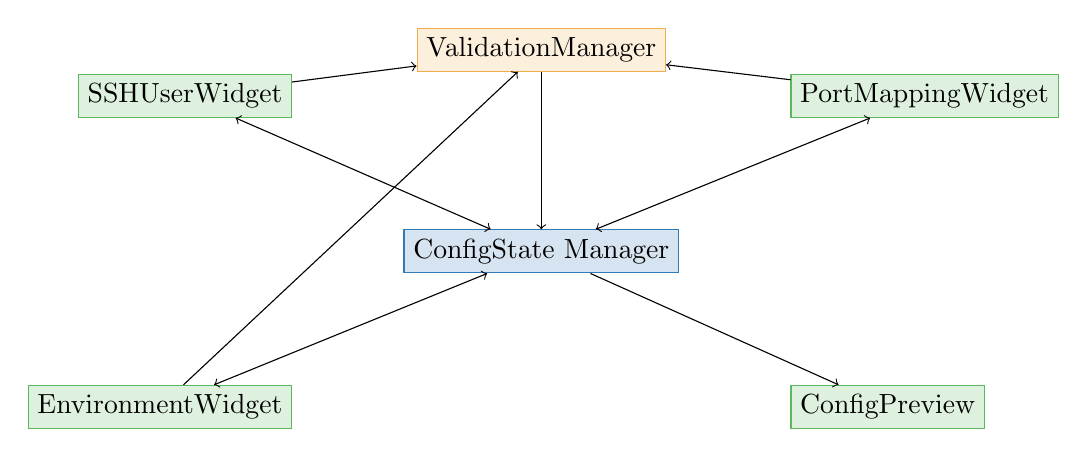
\begin{tikzpicture}[node distance=2cm]

% Central state manager
\node[rectangle, draw=primaryblue, fill=primaryblue!20] (state) {ConfigState Manager};

% Component widgets around the state manager
\node[rectangle, draw=successgreen, fill=successgreen!20, above left=of state] (ssh) {SSHUserWidget};
\node[rectangle, draw=successgreen, fill=successgreen!20, above right=of state] (ports) {PortMappingWidget};
\node[rectangle, draw=successgreen, fill=successgreen!20, below left=of state] (env) {EnvironmentWidget};
\node[rectangle, draw=successgreen, fill=successgreen!20, below right=of state] (preview) {ConfigPreview};

% Bidirectional arrows showing data flow
\draw[<->] (ssh) -- (state);
\draw[<->] (ports) -- (state);  
\draw[<->] (env) -- (state);
\draw[->] (state) -- (preview);

% Validation flow
\node[rectangle, draw=warningorange, fill=warningorange!20, above=of state] (validator) {ValidationManager};
\draw[->] (ssh) -- (validator);
\draw[->] (ports) -- (validator);
\draw[->] (env) -- (validator);
\draw[->] (validator) -- (state);

\end{tikzpicture}
\caption{Component Communication Architecture}
\end{figure}

\subsection{CSS Styling Specifications}

\begin{lstlisting}[caption={Component CSS Styles}, language=CSS]
/* Base widget styles */
BaseConfigWidget {
    border: solid $primary;
    background: $surface;
    padding: 1;
    margin: 1;
}

BaseConfigWidget.valid {
    border: solid $success;
}

BaseConfigWidget.invalid {
    border: solid $error;
}

/* Input widget styles */
ValidatedInput {
    border: solid $secondary;
    background: $surface;
}

ValidatedInput.valid {
    border-right: solid $success;
}

ValidatedInput.invalid {
    border-right: solid $error;
}

ValidatedInput:focus {
    border: solid $accent;
}

/* File path input styles */
FilePathInput {
    layout: horizontal;
}

FilePathInput.path-exists {
    border-left: solid $success;
}

FilePathInput.path-missing {
    border-left: solid $warning;
}

FilePathInput.path-invalid {
    border-left: solid $error;
}

FilePathInput.auto-discovery {
    color: $accent;
    text-style: italic;
}

/* Configuration widget styles */
SSHUserWidget {
    border: solid $primary;
    background: $surface-lighten-1;
    padding: 1;
}

PortMappingWidget {
    border: solid $primary;
    background: $surface-lighten-1;
}

PortMappingWidget ListView {
    border: solid $secondary;
    background: $surface;
}

PortMappingWidget ListItem:hover {
    background: $primary-darken-3;
}

/* Preview widget styles */
ConfigPreview {
    border: solid $secondary;
    background: $surface-darken-1;
    color: $text;
}

ConfigPreview.syntax-yaml {
    text-style: none;
}

/* Status widget styles */
ValidationStatus.valid {
    color: $success;
    text-style: bold;
}

ValidationStatus.warning {
    color: $warning;
    text-style: bold;
}

ValidationStatus.error {
    color: $error;
    text-style: bold;
}

/* Progress and loading styles */
ProgressIndicator {
    border: solid $accent;
    background: $surface;
}

ProgressIndicator > Bar {
    color: $accent;
}

/* Help and tooltip styles */
HelpDialog {
    border: solid $primary;
    background: $surface-lighten-2;
    color: $text;
    padding: 2;
}

Tooltip {
    border: solid $secondary;
    background: $surface-darken-2;
    color: $text-muted;
    padding: 1;
}
\end{lstlisting}

\subsection{Component Testing Specifications}

\begin{lstlisting}[caption={Component Testing Framework}]
import pytest
from textual.app import App
from textual._testing import TxtualTestCase
from pei_docker.gui.components import SSHUserWidget, PortMappingWidget

class TestSSHUserWidget(TxtualTestCase):
    """Test cases for SSH user configuration widget."""
    
    async def test_ssh_user_widget_creation(self):
        """Test SSH user widget initialization."""
        widget = SSHUserWidget(username="testuser")
        assert widget.username == "testuser"
        assert widget.config_key == "ssh_user"
        
    async def test_ssh_user_validation(self):
        """Test SSH user input validation."""
        widget = SSHUserWidget()
        
        # Test valid configuration
        widget.query_one("#username", Input).value = "testuser"
        widget.query_one("#password", Input).value = "validpass"
        widget.query_one("#uid", Input).value = "1100"
        
        result = widget.validate()
        assert result["valid"] is True
        assert len(result["errors"]) == 0
        
    async def test_ssh_user_invalid_uid(self):
        """Test SSH user UID validation."""
        widget = SSHUserWidget()
        
        # Test invalid UID
        widget.query_one("#username", Input).value = "testuser"
        widget.query_one("#password", Input).value = "validpass"
        widget.query_one("#uid", Input).value = "not_a_number"
        
        result = widget.validate()
        assert result["valid"] is False
        assert any("UID must be a valid number" in error for error in result["errors"])
        
    async def test_ssh_user_config_generation(self):
        """Test configuration data generation."""
        widget = SSHUserWidget()
        
        widget.query_one("#username", Input).value = "testuser"
        widget.query_one("#password", Input).value = "testpass"
        widget.query_one("#uid", Input).value = "1100"
        
        config = widget.get_config_data()
        expected = {
            "testuser": {
                "password": "testpass",
                "uid": 1100
            }
        }
        assert config == expected

class TestPortMappingWidget(TxtualTestCase):
    """Test cases for port mapping widget."""
    
    async def test_port_mapping_validation(self):
        """Test port mapping string validation."""
        widget = PortMappingWidget()
        
        # Test valid single port
        result = widget.validate_port_mapping("8080:80")
        assert result["valid"] is True
        
        # Test valid port range
        result = widget.validate_port_mapping("8000-8010:3000-3010")
        assert result["valid"] is True
        
        # Test invalid format
        result = widget.validate_port_mapping("invalid:mapping")
        assert result["valid"] is False
        
    async def test_port_mapping_addition(self):
        """Test adding port mappings."""
        widget = PortMappingWidget()
        initial_count = len(widget.port_mappings)
        
        # Simulate adding a port mapping
        widget.query_one("#port_input", Input).value = "9090:90"
        await widget.on_button_pressed(MockButtonEvent("add_port"))
        
        assert len(widget.port_mappings) == initial_count + 1
        assert "9090:90" in widget.port_mappings

# Mock classes for testing
class MockButtonEvent:
    def __init__(self, button_id: str):
        self.button = MockButton(button_id)
        
class MockButton:
    def __init__(self, button_id: str):
        self.id = button_id
\end{lstlisting>

\section{Component Documentation and Usage Guidelines}

\subsection{Development Guidelines}

\begin{enumerate}
    \item \textbf{Inheritance Pattern}: All configuration widgets must inherit from \texttt{BaseConfigWidget}
    \item \textbf{Validation}: Implement comprehensive validation with user-friendly error messages
    \item \textbf{Accessibility}: Support keyboard navigation and screen reader compatibility
    \item \textbf{Responsiveness}: Design widgets to work across different terminal sizes
    \item \textbf{Testing}: Provide comprehensive unit tests for all widget functionality
    \item \textbf{Documentation}: Include help text and tooltips for all configuration options
\end{enumerate}

\subsection{Performance Considerations}

\begin{itemize}
    \item \textbf{Lazy Loading}: Load widget content only when displayed
    \item \textbf{Debounced Validation}: Avoid excessive validation calls during rapid input
    \item \textbf{Efficient Updates}: Use reactive properties to minimize unnecessary re-renders
    \item \textbf{Memory Management}: Properly clean up widget resources on disposal
\end{itemize}

\end{document}